%
% Another appendix chapter
\chapter{Theoretic Limits on Capture}
In this chapter there is looked at the point foot - point mass model, so no angular momentum is included.\\
This chapter matches the goal of exploring the effects of height variation.\\
A common habit is to formulate an optimization problem, and to `let the optimization figure it out', but there is not looked at limits.\\
In the point-foot, point-mass model with prismatic leg joint, the constraints are:
\begin{itemize}
	\item Unilateral ground reaction force
	\item Limit on leg length
	\item Limit on leg force
	\item Limit on ground friction
\end{itemize}

 %% Capture Region
\section{Unconstrained Capture Region}
In this section the bounds are given with respect to capturability of a horizontal traveling CoM, like with the study of the capture point. The only constraint taken into account is unilaterality of \ac{GRF}. Also a measure of this limit is given in terms of the CP.\\
Balistic touchdown time for a given height is:
\begin{equation}
	t = \sqrt{\frac{2z_0}{g}}
\end{equation}
The horizontal location is:
\begin{equation}
	x_{balistic}= \dot{x}t=\dot{x}\sqrt{\frac{2z_0}{g}} 
\end{equation}
which is then compares to the capture point as:
\begin{equation}
    x_{balistic}=\sqrt{2}x_{cp}
\end{equation}
This can also be reasoned from a leg force perspective, as no energy is substracted from the CoM during its travel. \\
Using this formulation of the problem and \Elip:
\begin{equation}
   x_{balistic}^2 = \frac{z_0}{g}(\dot{x}_0^2 + \dot{x}_f^2) 
\end{equation}
Capture limits: leg can apply an infinite force just after the current position to stop on that horizontal location. The other side of the bound is the balistic touch down point, where the virtual leg can apply an impact when the mass hits the ground equal to its velocity and in the direction, then lift the mass up to the desired or default height. This limit on the capture region is defined as:
\begin{equation}
\{x_{cp} \in (0, \dot{x}\sqrt{\frac{2z_0}{g}} ]\}
\end{equation}
\cite{koolen2016balance} \figref{fig:cpbal}
\begin{figure}[h]
\centering
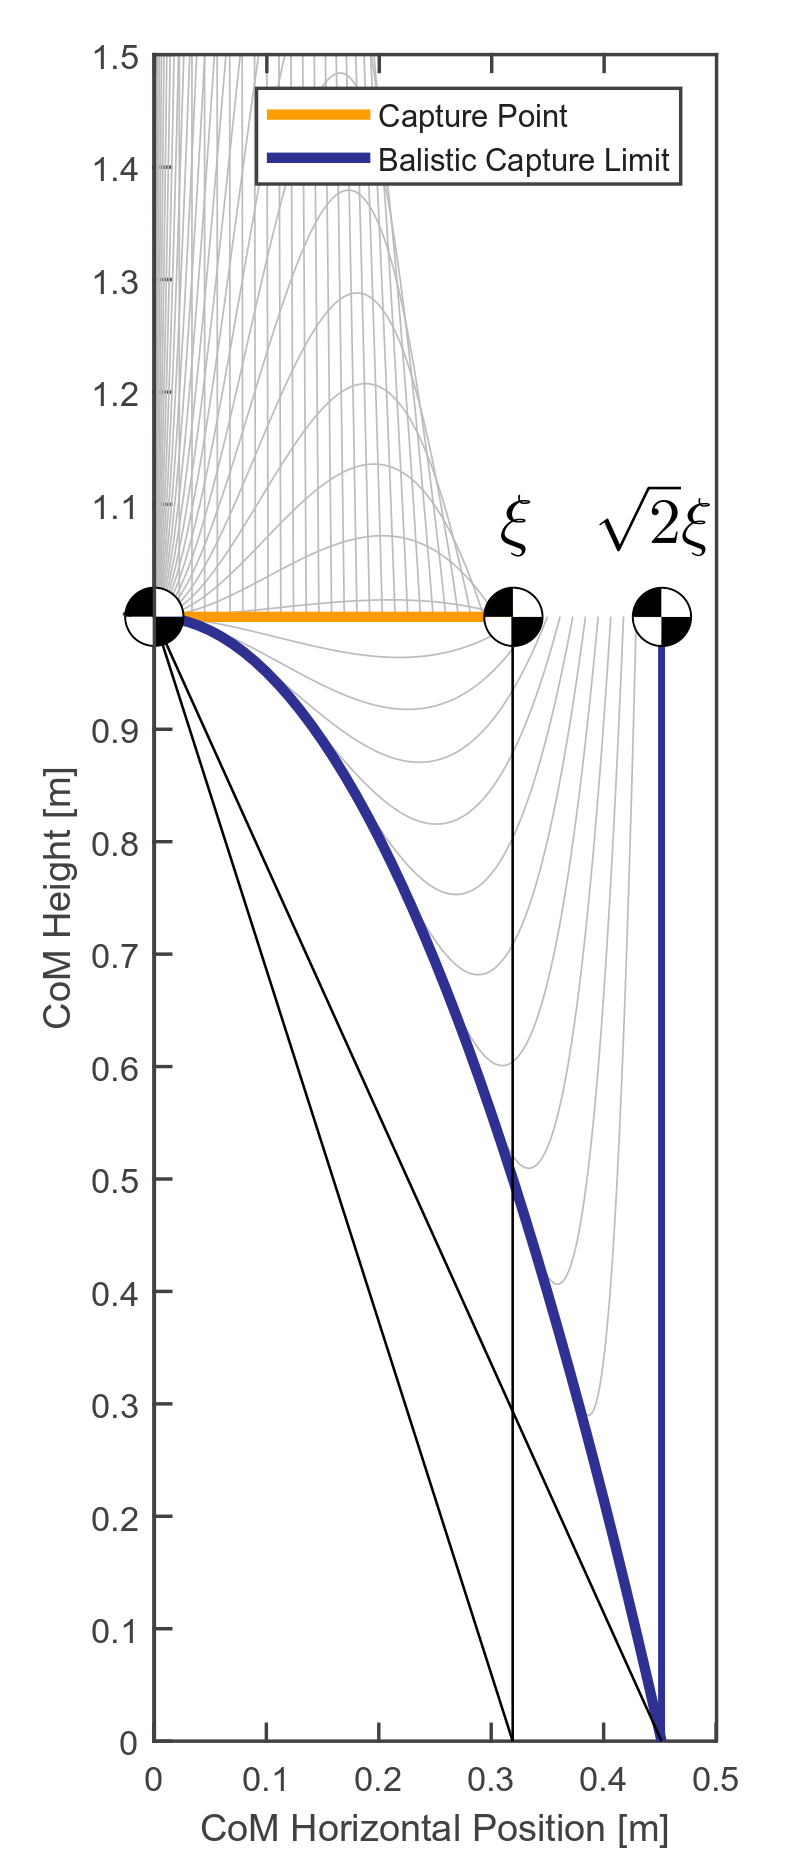
\includegraphics[width=0.3\textwidth]{STYLESTUFF/CPvsBalistic.png}
\caption{Unconstrained capture region and balistic limit, grey plots visualize intermediate trajectories and are made with the method of \cite{koolen2016balance}}
\label{fig:cpbal}
\end{figure}

%% Height Constrained
\section{Height Constrained Capture}
No leg length constriant, but height constraint. \figref{fig:cpheight}
\begin{equation}
    x_{cp,height}=(\frac{\sqrt{2g\delta z_{max}}}{g}+\sqrt{\frac{z_o+\delta z_{max}}{g}})(\dot{x}_0-\frac{x_0}{z_0}\sqrt{2g\delta z_{max}}).
\end{equation}
\begin{figure}[h]
\centering
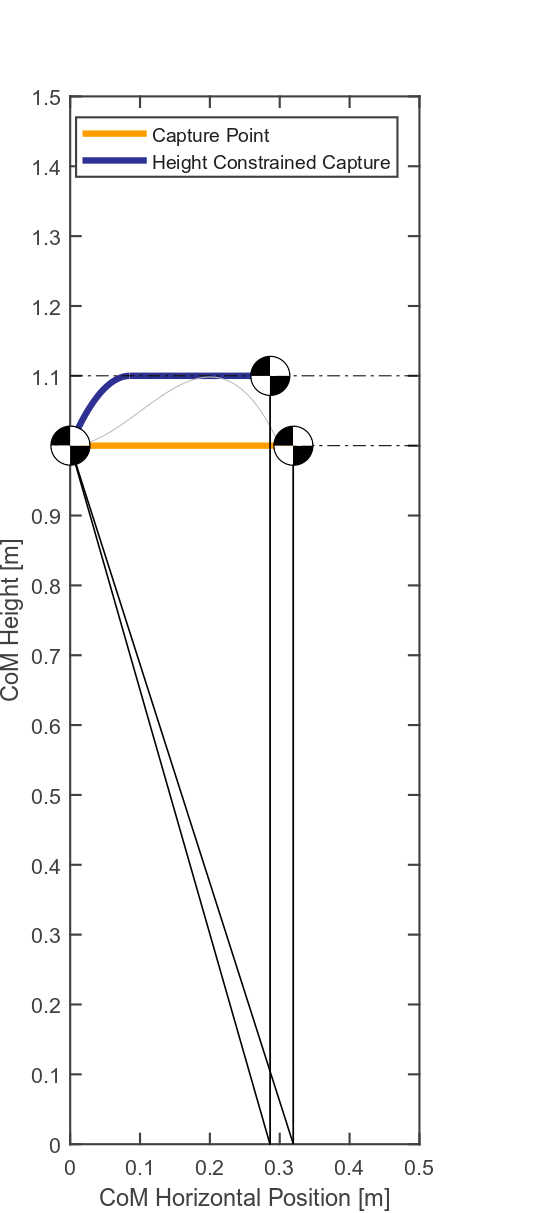
\includegraphics[width=0.3\textwidth]{STYLESTUFF/CPvsHeight.png}
\caption{Height constrained capture limit. Grey plot is made with the method of \cite{koolen2016balance} and shows that the final point lies between the limit and the \ac{CP}}
\label{fig:cpheight}
\end{figure}

\section{Impact Influenced Capture}
\begin{equation}
x_{cp,impact} = \sqrt{\frac{z}{g}}(\dot{x}+\dot{x}_I)
\end{equation}

\begin{equation}
x_{cp,impact} = \sqrt{\frac{z}{g}}(\dot{x}+\frac{x}{z}\dot{z})
\end{equation}

\begin{equation}
x_{cp,impact} = \frac{z}{\sqrt{zg}-\dot{z}}
\end{equation}
\cite{kuo2005energetic}, mention also straight leg walking, planning.